\newpage
\section{Results and discussion}\label{results}
This section presents the results of the Austrian case study in 2050. The focus is put on the mix of heat sources/generation technologies and district heating in the four different scenarios. Section \ref{results1} shows the heat supply of a representative Austrian NUTS3 region in detail. Building upon, section \ref{results2} compares heat supply in an urban and a rural LAU/district. Section \ref{results3} presents the obtained heat densities of district heating networks. Finally, section \ref{results4} syntheses the results of district heating and provides indications/information that could be returned into more aggregate models, such as GENeSYS-MOD, in the sense of a feedback loop.

\subsection{Heat supply in a representative NUTS3 region in 2050}\label{results1}
This section presents the results of the NUTS3 region 'Salzburg and Surroundings' (AT323). Figure \ref{fig:1} shows the most relevant results in this region on LAU/district level for the four different scenarios. District heating supplies heat demands in 5 different LAUs/districts. In particular, the LAUs are in the surrounding area of Salzburg city (marked by the star). The remaining LAUs in the NUTS3 region are supplied decentralized/on-site. Details of the heat sources that supply heat demands in LAUs with district heating and with decentralized/on-site heat systems are presented in the following section \ref{results2}. The amount of district heating varies between \SI{1,045}{} and \SI{1,132}{TWh} per year (Figure \ref{fig:1}, top right). The highest value is achieved in the Gradual Development scenario since this is the scenario with the lowest heat demand reduction. The heat density of district heating in the 5 LAUs is shown in Figure \ref{fig:1}, bottom right. The highest heat density is achieved in Salzburg city and reaches approximately \SI{30}{GWh\per km^2} in each scenario. The comparable low heat densities in two of the five LAUs (marked by rectangle and plus) is further discussed in section \ref{results4}. 

\begin{figure}[h]
	\centering
	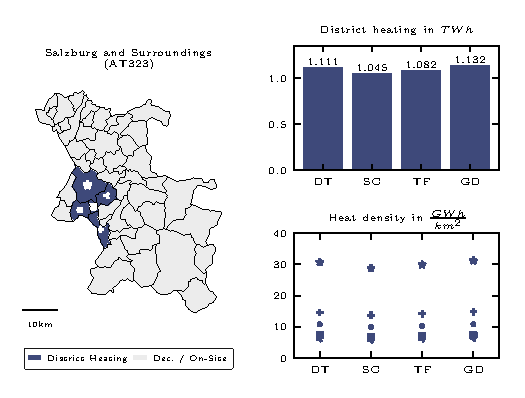
\includegraphics[width=1\linewidth]{figures/lau-networks/network-salzburg.eps}
	\caption{District heating and decentralized/on-site heat supply in the representative NUTS3 region (incl. LAUs/districts) 'Salzburg and Surroundings' (AT323). Left: LAUs with district heating or on-site heat supply. Top right: Total amount of district heating in the four different scenarios. Bottom right: heat density of district heating in the four different scenarios.}
	\label{fig:1}
\end{figure}

\subsection{Comparison of heat supply in urban and rural LAUs/districts}\label{results2}
Building upon the so-far presented results of the NUTS3 region 'Salzburg and Surroundings', this section shows the heat sources/generation technologies supplying heat demands in an urban and in a rural LAU/district. We use 'Salzburg' city (urban district) and 'Abtenau' (rural district) as representative LAUs. Figure \ref{fig:2} shows the mix of heat sources supplying heat demands in both LAUs. The geographical location is shown on the top left in Figure \ref{fig:2}. In 'Salzburg' city (marked by the orange edge), district heating supplies heat demands, which uses large-scale heat pumps (air-sourced), hydrogen, synthetic gas, and waste as heat sources/generation technologies. High shares of district heating particularly are generated by large-scale heat pumps (air) and using hydrogen. In contrary, the heat supply in the rural district 'Abtenau' uses small-scale heat pumps (air), heat pumps (ground-sourced), biomass, and direct electric heating systems. Among all four scenarios, high shares of heat demands are supplied by heat pumps (air- and ground-sourced). However, the share of each technologies varies to some extent significantly, which becomes evident when comparing exemplarily the Techno-Friendly and Gradual Development scenario. In the Techno-Friendly, small-scale heat pumps (air-sourced) are the dominant heat source, whereby heat pumps (ground-sourced) supply high shares of heat demands in the Gradual Development scenario.

\begin{figure}[h]
	\centering
	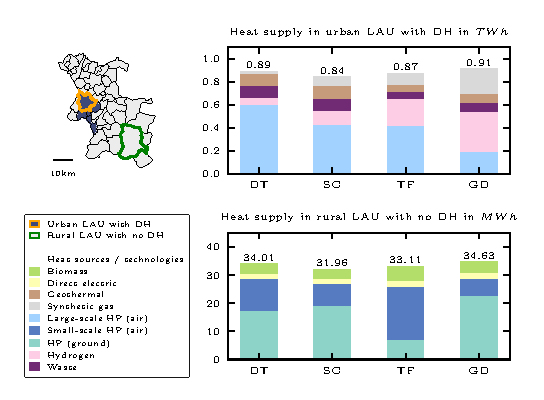
\includegraphics[width=1\linewidth]{figures/lau-supply/supply-salzburg-lau.eps}
	\caption{Comparison of heat supply in an urban LAU with district heating ('Salzburg' city) and in a rural LAU with no district heating ('Abtenau'). Top right: Mix of heat sources in the four different scenarios used in district heating. Bottom right: Mix of heat sources used to supply heat demands decentralized/on-site.}
	\label{fig:2}
\end{figure}

\subsection{Heat densities of district heating in LAUs in 2050}\label{results3}
This section shows the heat density of district heating at the LAU/district level in 2050. Figure \ref{fig:3} shows the heat density for the four different scenarios. Particularly, the values of LAU's heat densities are sorted in descending order indicating those LAUs/districts that do not reach the required heat density of economic viability, which is assumed to be \SI{10}{GWh \per km^2}. Exemplarily, in the Directed Transition scenario, there are 107 LAUs with district heating. In this scenario, the highest heat density is \SI{43.17}{GWh \per km^2}. 2 of the 5 LAUs in the NUTS3 region 'Salzburg and Surroundings' are highlighted, namely, 'Salzburg' city (marker by the star in Figure \ref{fig:1}) and 'Anif' (marked by the rectangle in Figure \ref{fig:1}). Both LAUs are part of the same district heating network as already illustrated in the left subfigure in Figure \ref{fig:1}. Accordingly, the appearance of heat densities below the assumed threshold/benchmark for economic viability can be argued as those LAUs are connected to high heat density areas. The distribution of heat density values remains mostly the same between the four different scenarios. For the sake of clarity, explicit annotations are omitted in the three (smaller) scenario subfigures at the bottom. 

\begin{figure}[h]
	\centering
	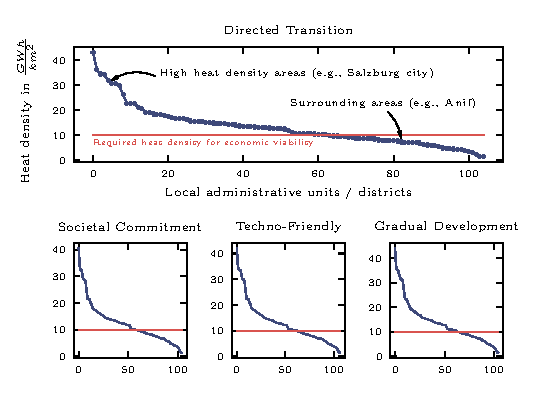
\includegraphics[width=1\linewidth]{figures/heat-density-duration-curve/heat-density-duration.eps}
	\caption{Heat density values at the LAU level in the four different scenarios in descending order indicating those LAUs that do not achieve the required heat density benchmark for economic viability.}
	\label{fig:3}
\end{figure}

\subsection{Comparison of heat supply in urban and rural districts}\label{results4}
We focus in this section on those LAUs with lower heat densites than assumed to be required for economic viability for district heating and their geographical location in respect to other district heating supply areas. As indicated in Figure \ref{fig:3}, LAUs with low heat densities can be quite justified in case that they are located in the surrounding area of high heat density areas (e.g., Salzburg city and Anif). However, other LAUs that do not achieve the required heat density benchmark (of \SI{10}{GWh \per km^2}) and at the same time are not closely located to high heat density areas are unlikely to be implemented. Accordingly, Figure \ref{fig:4} shows the heat map of district heating in Austria at the LAU level under the requirement that district heating achieves the required heat density benchmark within NUTS3 regions in the Directed Transition scenario. As previously mentioned, the model basically decides to supply heat demands in 105 LAUs by district heating. 63 of them already achieved heat densities higher than the benchmark value. The heat map in Figure \ref{fig:4} still shows 68 LAUs since 5 are closely located to high heat density areas and thus achieve in total the benchmark (at the NUTS3 level). 

\begin{figure}[h]
	\centering
	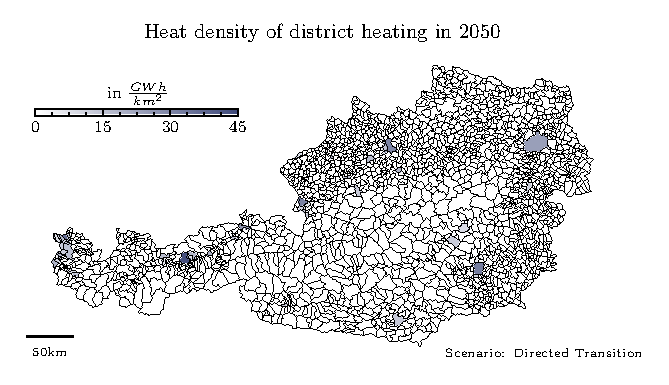
\includegraphics[width=1\linewidth]{figures/austria-heat-density/austria-laus.eps}
	\caption{Heat density of district heating in the Directed Transition scenario in 2050 achieving the required heat density benchmark value of \SI{10}{GWh \per km^2} at the NUTS3 level.}
	\label{fig:4}
\end{figure}

Accordingly, district heating is unlikely to be implemented in 37 LAUs. Table \ref{tab:overview} summarizes the results for district heating in the four different scenarios. It is shown that as a result of the heat density benchmark at the NUTS3 level the share of implemented district heating varies between 74 and 90\%. In particular, this means exemplarily that in the Techno-Friendly scenario, 74\% of the assumed heat supply using district heating leads to heat density values higher than \SI{10}{GWh \per km^2}. In view of the previous assumptions that 50\% of heat pumps (air-sourced) are used in district heating, this results in implemented shares between 23\% and 40\%, whereby the highest share is achieved in the Directed Transition scenario. 



\definecolor{Gray}{gray}{0.95}
\begin{table}[h]
	\centering
	\scalebox{0.875}{
		\renewcommand{\arraystretch}{1.35}
		\begin{tabular}{lrrrr}
			\toprule 
			Results in the four scenarios (from Sec. \ref{res:1}) & DT & SC & TF & GD\\\hline
			District Heating (from GENeSYS-MOD) in TWh & 16.75 & 15.38 & 27.20 & 22.84\\
			LAUs with district heating (from downscaling) & 105 & 105 & 107 & 105\\
			- of which with more than \SI{10}{GWh \per km^2} & 63 & 57 & 62 & 64\\
			- of which with less than \SI{10}{GWh \per km^2} & 42 & 60 & 45 & 41\\
			LAUs with district heating (\SI{10}{GWh \per km^2} at NUTS3) & 68 & 66 & 68 & 68\\
			\cellcolor{Gray}District heating (\SI{10}{GWh \per km^2} at NUTS3) in TWh & \cellcolor{Gray}14.57  & \cellcolor{Gray}13.08 & \cellcolor{Gray}20.09 & \cellcolor{Gray}20.62\\
			- share in district heating from GENeSYS-MOD in \% & 87 & 85 & 74 &90\\
			- share of large-scale heat pumps (air) in \% & 40 & 35 & 23 & 26 \\\bottomrule
	\end{tabular}}
	\caption{Overview of district heating supplying heat demands in 2050 in the four different scenarios Directed Transition (DT), Societal Commitment (SC), Techno-Friendly (TF), and Gradual Development (GD). The resulting district heating that reaches the heat density benchmark of \SI{10}{GWh \per km^2} at the NUTS3 level is marked in gray.}
	\label{tab:overview}
\end{table}

In view of the underlying narratives of particularly the three ambitious decarbonization scenarios from Section \ref{res:1} (therefore excluded the Gradual Development scenario), two interesting implications can be derived from the results here:
\begin{itemize}
	\item In absolute terms, the Techno-Friendly scenario has the highest share of district heating with \SI{20.09}{TWh} under the condition that district heating networks within the NUTS3 levels achieve the heat density benchmark of \SI{10}{GWh \per km^2}. The main driver for this is the significant penetration of (large-scale) heat pumps (air-sourced) that takes place in this scenario.
	\item Nevertheless, the implemented share of district heating in GENeSYS-MOD's district heating assumptions is the highest in the Directed Transition scenario and reaches \SI{87}{\%}. This result is also reflected in the fact that the share of large-scale heat pumps (air-sourced) achieves here its maximum with \SI{40}{\%}.
\end{itemize}

